\chapter{Convolutional Neural Network}
\label{cha:CNN}

The dataset consists of a training and a test dataset of MRI images of brain tumours. 
The training dataset is split into a training and a validation subset, containing 80\% and 20\% of the data, leading to 2408 and 602 samples, respectively.
The test dataset contains 752 samples.
The images are grayscale and have a size of $240 \times 240$ pixels.
No further preprocessing is applied to the data.
Malignant tumours are labelled as positive, while benign tumours are labelled as negative.
Therefore, a false negative prediction is a malignant tumour classified as benign, while a false positive prediction is a benign tumour classified as malignant.
The goal is to classify the tumours with a bias towards the malignant tumours, as it is much more dangerous for a patient to have a malignant tumour classified as benign than vice versa.
Recall is used as the main metric to evaluate the models to reflect this.
% It is the ratio of the true positive benign tumours to the sum of the true positive benign tumours and the false negative malignant tumours.
During the training, however, the model is optimized using the accuracy.
% The recall is defined as the ratio of the true positive predictions to the sum of the true positive and false negative predictions.
% Benign tumours are labelled as the positive class, while malignant tumours are labelled as the negative class.
% In that way, the model should have a bias towards the malignant tumours.
% The accuracy, the precision, the F1-score, the $R^2$-score, the mean squared error, and the mean absolute error are also calculated.
Further metrics are calculated to evaluate the models. \newline
The CNN is implemented using the Keras \cite{keras} library with a TensorFlow \cite{tensorflow} backend.
The plots are created using the matplotlib, the pandas, and the seaborn libraries \cite{matplotlib, pandas, seaborn}.
Additionally, the numpy library is used \cite{numpy}.

\section{Network Architecture and Initial Model}
\label{sec:initialModel}

The CNN starts with a rescaling layer, which scales the grayscale to the range of $[0, 1]$.
It is followed by three convolutional layers with 24, 12 and 8 filters respectively, a kernel size of $3 \times 3$ and a stride of 1.
Each convolutional layer is followed by a max-pooling layer with a pool size of $2 \times 2$.
The convolutions are followed by a flattening layer, which converts the 2D output of the convolutional layers to a 1D array.
% To reduce overfitting, a dropout layer with a dropout rate of 0.5 is added.
Two dense layers with 4 and 2 neurons are added, respectively.
The last dense layer serves as the output layer.
The activation function used in every layer is the rectified linear unit (ReLU).
The CNN is trained to minimize the sparse categorical cross-entropy loss using the Adam optimizer \cite{adam} with a batch size of 32 images.
The model is trained for 30 epochs.
After multiple runs of the initial model, it was observed that the model was overfitting.
This was indicated by the large difference between the training and validation accuracy.
To reduce overtraining, a dropout layer with a dropout rate of 0.5 was added to the model and the learning rate of the Adam optimizer was also increased from $0.001$ to $0.005$.
In total, 29,250 parameters can be trained in this architecture.
\begin{figure}[H]
    \centering
    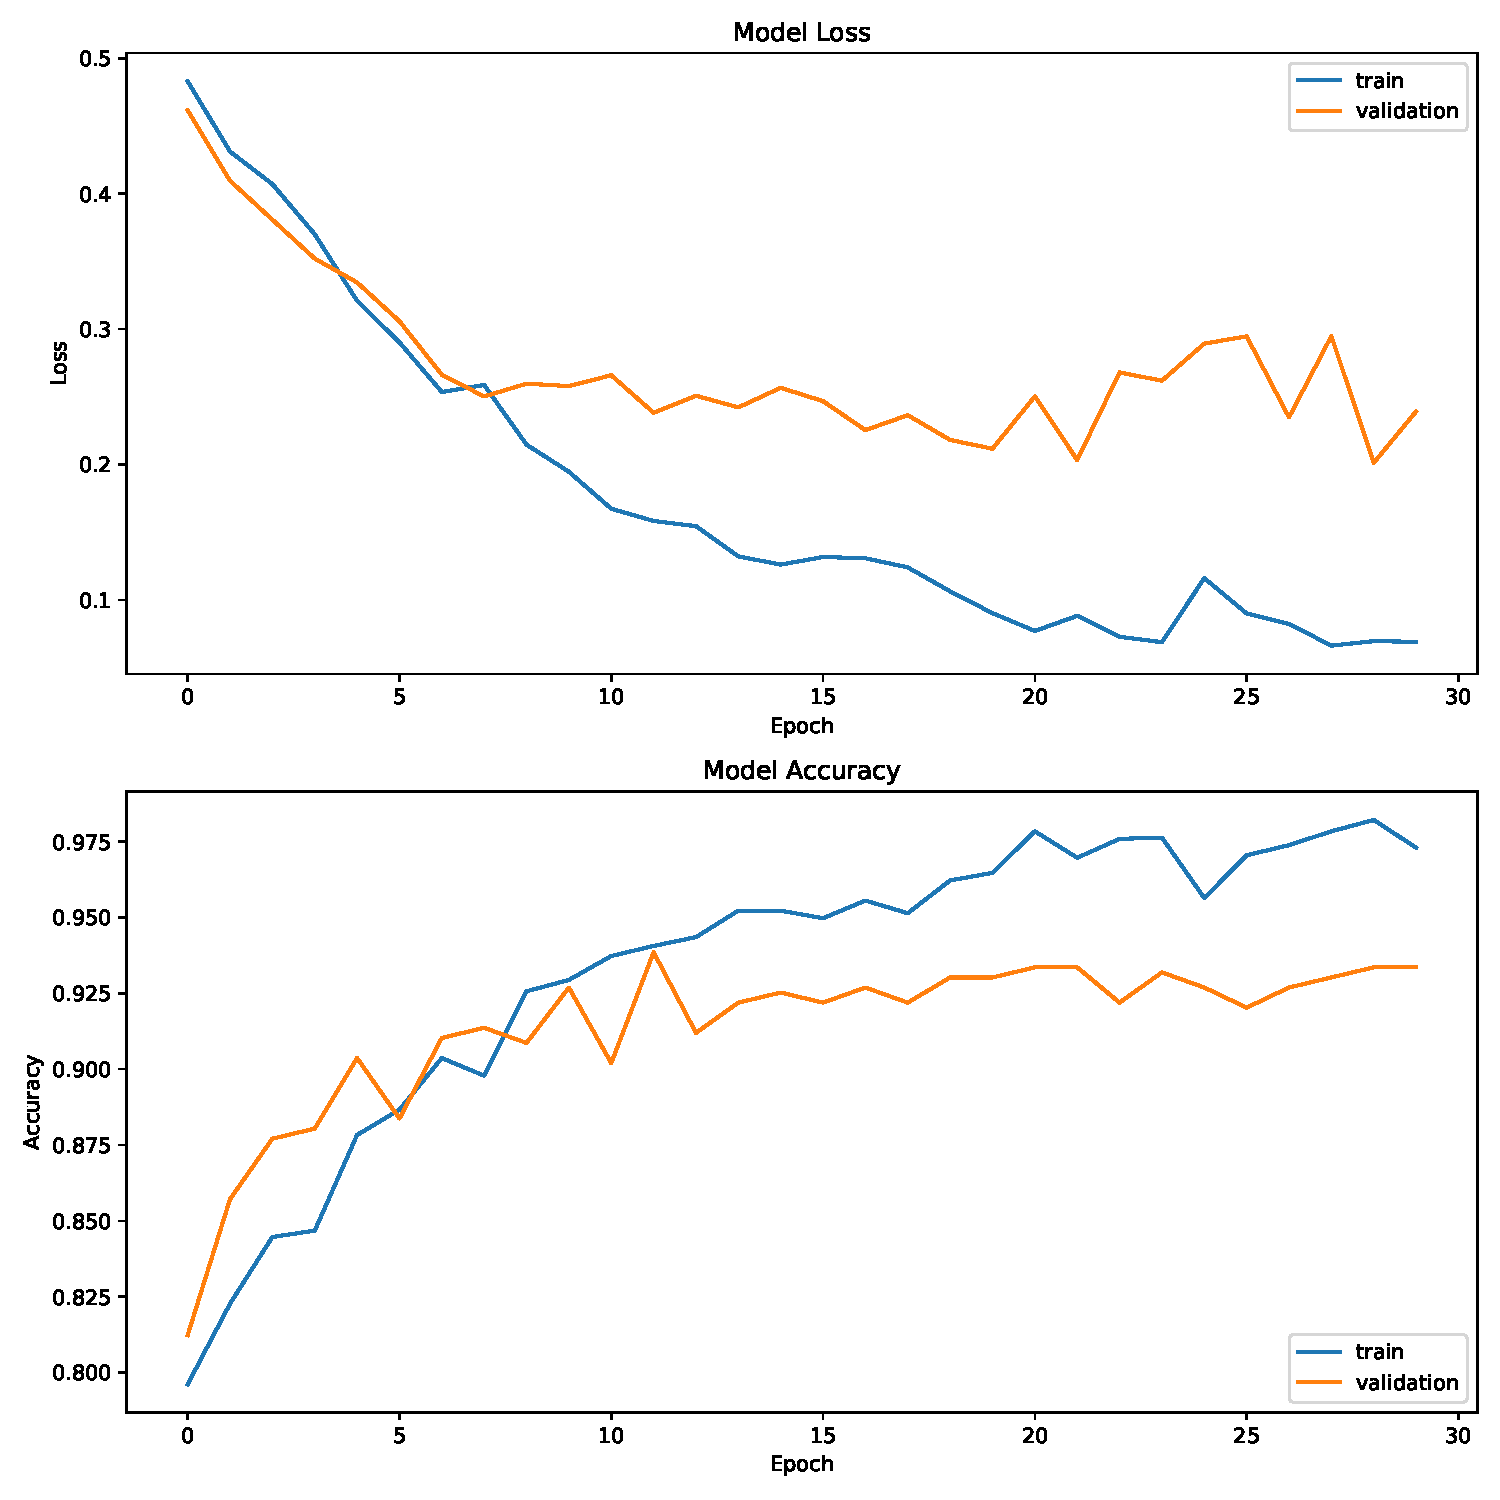
\includegraphics[width=.65\textwidth]{plots/Initial-history.pdf}
    \caption{Accuracy- and loss-curves for the initial CNN.}
    \label{fig:learningCurveInitial}
\end{figure}
\begin{wrapfigure}{r}{5cm}
    \centering
    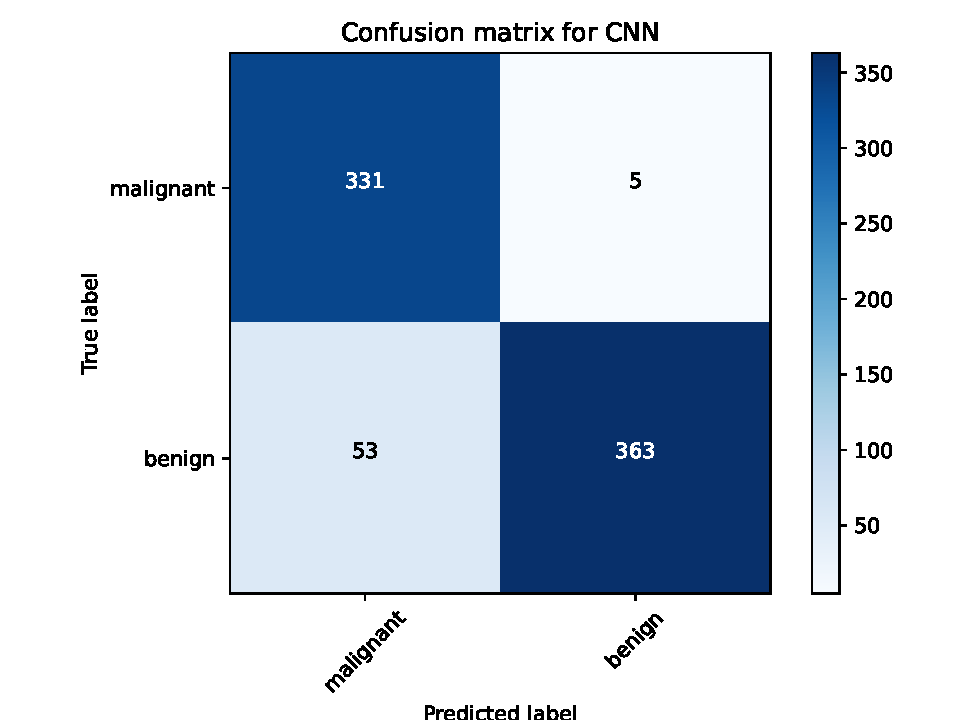
\includegraphics[width=.48\textwidth]{plots/confusion_matrix_CNN.pdf}
    \caption{Confusion matrix for the initial CNN.}
    \label{fig:confusionMatrixInitial}
    \rule{4cm}{0cm}
\end{wrapfigure}
The model was retrained for 30 epochs and the accuracy- and loss-curves are shown in figure \ref{fig:learningCurveInitial}.
The learning curves show a high accuracy already, but the model is still overfitting as can be seen by the diverging training and validation loss beginning at around the 13th epoch.
\newline
To further investigate the model, a confusion matrix was created, which is shown in figure \ref{fig:confusionMatrixInitial}.
The confusion matrix shows that the model has a high accuracy for the benign tumours, but a low accuracy for the malignant tumours.
It classifies more benign tumours as malignant than vice versa. %, which is the desired behaviour.
This reflects the bias towards the malignant tumours that was desired.
% The metrics for the initial model are shown in the summary below.
The model has a recall value of 87.26\%, which means that 58 tumours are wrongly classified in the test dataset of 752 samples.
This is not sufficient enough for a medical application in such a critical field.
Additionally to the recall and accuracy, the precision, the f1-score, the $R^2$-score and the mean squared error are calculated and the metrics are shown in the summary below.
\begin{align}
    \label{eq:metricsInitialCNN}
    \begin{split}
        \text{recall} &= 0.8726, \\
        \text{accuracy} &= 0.9229, \\
        \text{precision} &= 0.9864, \\
        \text{f1-score} &= 0.9260, \\
        R^2\text{-score} &= 0.6880, \\
        \text{Mean Squared Error} &= 0.0771.
    \end{split}
\end{align}
It can be seen that the f1-score is 92.60\%, which reflects that the model is not good enough.
This is also evidenced by the $R^2$-score of 68.80\%, which indicates the model's efficacy in regressing to actual values.
% More importantly, the recall value of 87.26\% is not high enough as 58 tumours are wrongly classified, which is a lot in a test dataset of only 752 samples.
% More importantly, the recall value of 87.26\% is not satisfactory as 58 tumours are wrongly classified, which is a lot in a test dataset of only 752 samples.
% How good the model is at predicting the actual values is indicated by the $R^2$-score, which is 0.6880, which means it is off by 31.2\%.
These metrics can be improved by running the model for more epochs, but the problem of high overfitting needs to be resolved first to make the results more reliable and prevent the model from memorizing the training data.

\section{Hyperparameter Optimization}
\label{sec:hyperparameter}

To be able to know which of the hyperparameters lead to overfitting and which increase the performance the most, a grid search over a parameter space was performed by iterating over the number of filters in the convolutional layers, the dropout rate, and the number of dense layers.
The network architecture was kept the same as in the initial model, but the hyperparameters were varied. 
A preceding grid search was performed before the following one which led to the range of hyperparameters tested.
The preceding grid search is explained in section \ref{sec:FirstGridsearchHyperparameterTests}.
The number of filters in the first convolutional layer was $n_{\text{filters}}$ with $n_{\text{filters}} \in [24, 36, 48, 60, 72]$ with the second and third convolutional layers being $n_{\text{filters}}/2$ and $n_{\text{filters}}/3$, respectively.
The dropout rate $do$ was varied with $do \in [0.4, 0.5, 0.6]$ and the number of dense units $n_{\text{dense}}$ with $n_{\text{dense}} \in [4, 8, 12, 16, 20, 24]$.
The last layer was always a dense layer with 2 neurons.
The models were trained for 30 epochs and other hyperparameters were kept the same as in the initial model. \newline
The results of the grid search are shown in figure \ref{fig:gridsearch}.
It shows the effect of the individual hyperparameters on the best validation accuracy, the best training accuracy and the difference between both accuracies, denoted as delta accuracy.
The delta accuracy is calculated by subtracting the validation accuracy from the training accuracy and normalizing it by the validation accuracy.
\begin{figure}[H]
    \centering
    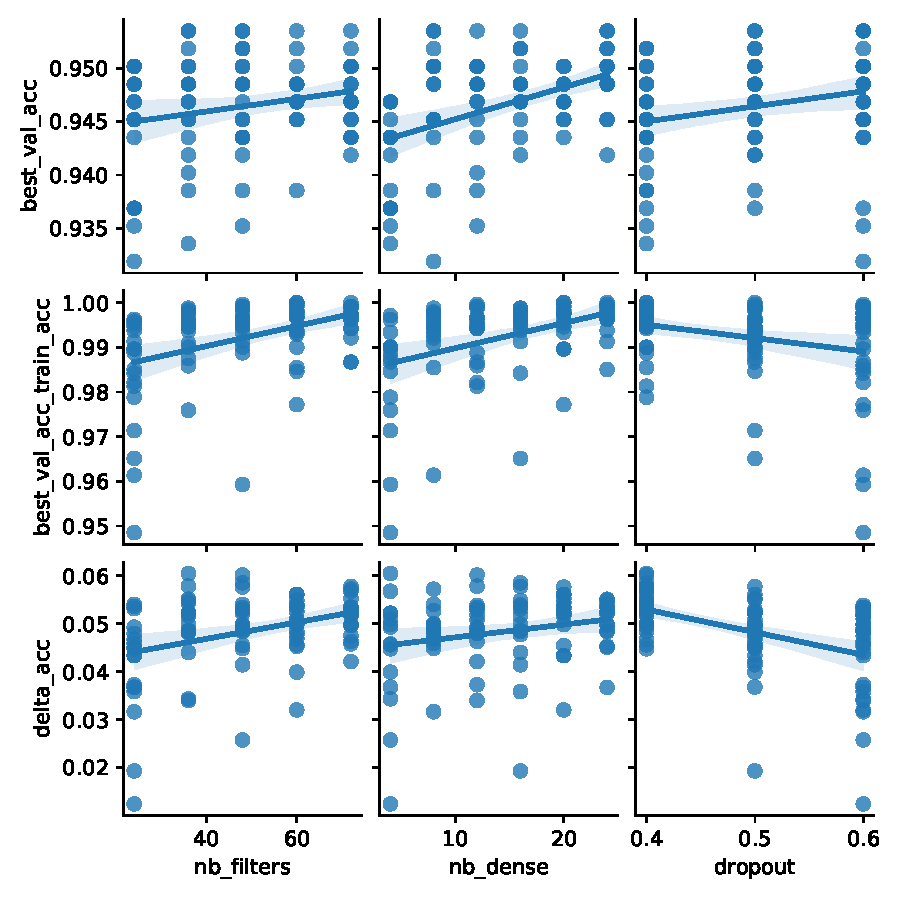
\includegraphics[width=0.65\textwidth]{plots/pairplot.pdf}
    \caption{Hyperparameter testing using a grid search.}
    \label{fig:gridsearch}
\end{figure}
% Figure \ref{fig:gridsearch} shows the effect of the individual hyperparameters on the best validation accuracy, the best training accuracy and the difference between the delta accuracy.

It can be seen that the training and the validation accuracy increase with an increase in the number of filters in the convolutional layers.
The effect is more pronounced for the training accuracy.
Increasing the number of filters, however, increases the delta, thus leading to more overfitting.
With an increase in dense units, the training and the validation accuracy also increase, with the more pronounced effect being on the validation accuracy.
The delta between the training and the validation accuracy also increases with an increase in dense units, but this effect is less distinctive than with the number of filters.
The dropout rate has a negative effect on the training accuracy and a positive effect on the validation accuracy.
Because of this behaviour, an increase in the dropout rate leads to a decrease in the delta accuracy. %, thus reducing overfitting.
This is because the dropout rate reduces the overfitting by randomly setting a fraction of the input units to 0 at each update during training.
The first grid search showed similar results, which is why in this grid search the range of dropout rates was increased to a maximum of 0.6 and the range of dense units was increased to a maximum of 24.
The number of filters was not increased, with the only difference being that more filters were tested. %\newline

Figure \ref{fig:gridsearchLearningCurves} shows the learning curves of the best three performing models with figure \ref{fig:SmallestDelta_LearningCurves} showing the models with the least difference in training and validation accuracy and figure \ref{fig:HighestAccuracyLearningCurves} showing the models with the highest accuracy.
\begin{figure}
    \centering
    \begin{subfigure}[B]{.45\textwidth}   % 1st subfigure
        \centering
        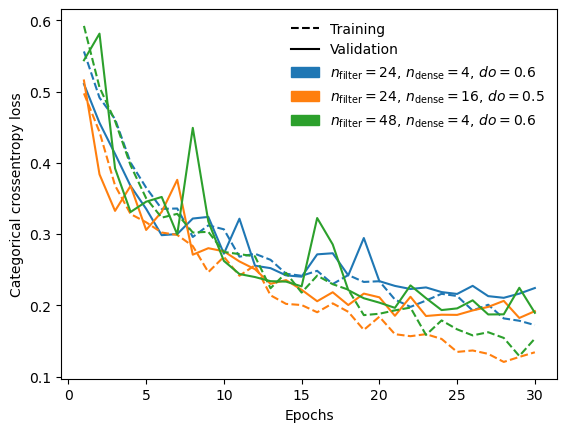
\includegraphics[width=\linewidth]{plots/SmallestDelta_LearningCurves.png}
        \caption{Learning curves of the models with the least difference in training and validation.}
        \label{fig:SmallestDelta_LearningCurves}
    \end{subfigure}    
    \begin{subfigure}[B]{.45\textwidth}   % 2nd subfigure
        \centering
        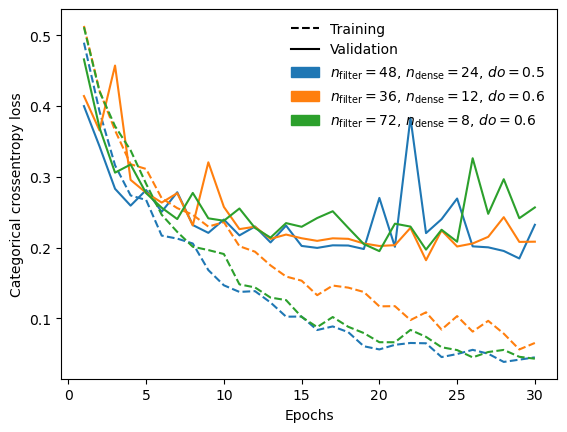
\includegraphics[width=\linewidth]{plots/Best3LearningCurves.png}
        \caption{Learning curves of the models with the highest accuracy.}
        \label{fig:HighestAccuracyLearningCurves}
    \end{subfigure}
    \caption{Learning curves of the models from the grid search.}
    \label{fig:gridsearchLearningCurves}
\end{figure}
What can be seen in figure \ref{fig:SmallestDelta_LearningCurves} is that the models with the least difference in delta accuracy seem like they are not trained enough.
The categorical cross-entropy loss is still decreasing, which means that the models could be trained for more epochs.
That the training and validation loss curves are so close to each other is a promising sign, as it means that the model is not overfitting as much as before and that there is still potential for improvement.
The model with the least amount of delta accuracy is also the least complex model with only 24 convolutional filters and 4 dense units.
The dropout rate is 0.6, which is the highest dropout rate tested.
This reflects the results from figure \ref{fig:gridsearch}, where the dropout rate had the most significant effect on the delta accuracy. \newline
The models with the highest accuracy, however, are already showing signs of overfitting, as can be seen in figure \ref{fig:HighestAccuracyLearningCurves}.
At around the same epoch as in the initial model, the training and validation loss curves start to diverge.
This means that the models are already overfitting and that they should not be trained for more epochs.
The reason for the large overfitting is due to the models being too complex for the amount of data available with the model with the highest accuracy having 48 convolutional filters and 24 dense units and only a dropout rate of 0.5.
The learning curves of the best three performing models in their respective categories in figure \ref{fig:gridsearchLearningCurves} confirm the results from the grid search in figure \ref{fig:gridsearch}.
The model with the least amount of delta accuracy is the one that is chosen for the final model as it shows the least amount of overfitting and still has potential for improvement.

\section{Final Model}
\label{sec:finalModel}

The final model is the model with the least amount of delta accuracy from the grid search and is trained for 100 epochs. % with the Adam optimizer and a learning rate of 0.005.
The learning curves for the final CNN are shown in figure \ref{fig:learningCurveFinal}.
\begin{figure}[H]
    \centering
    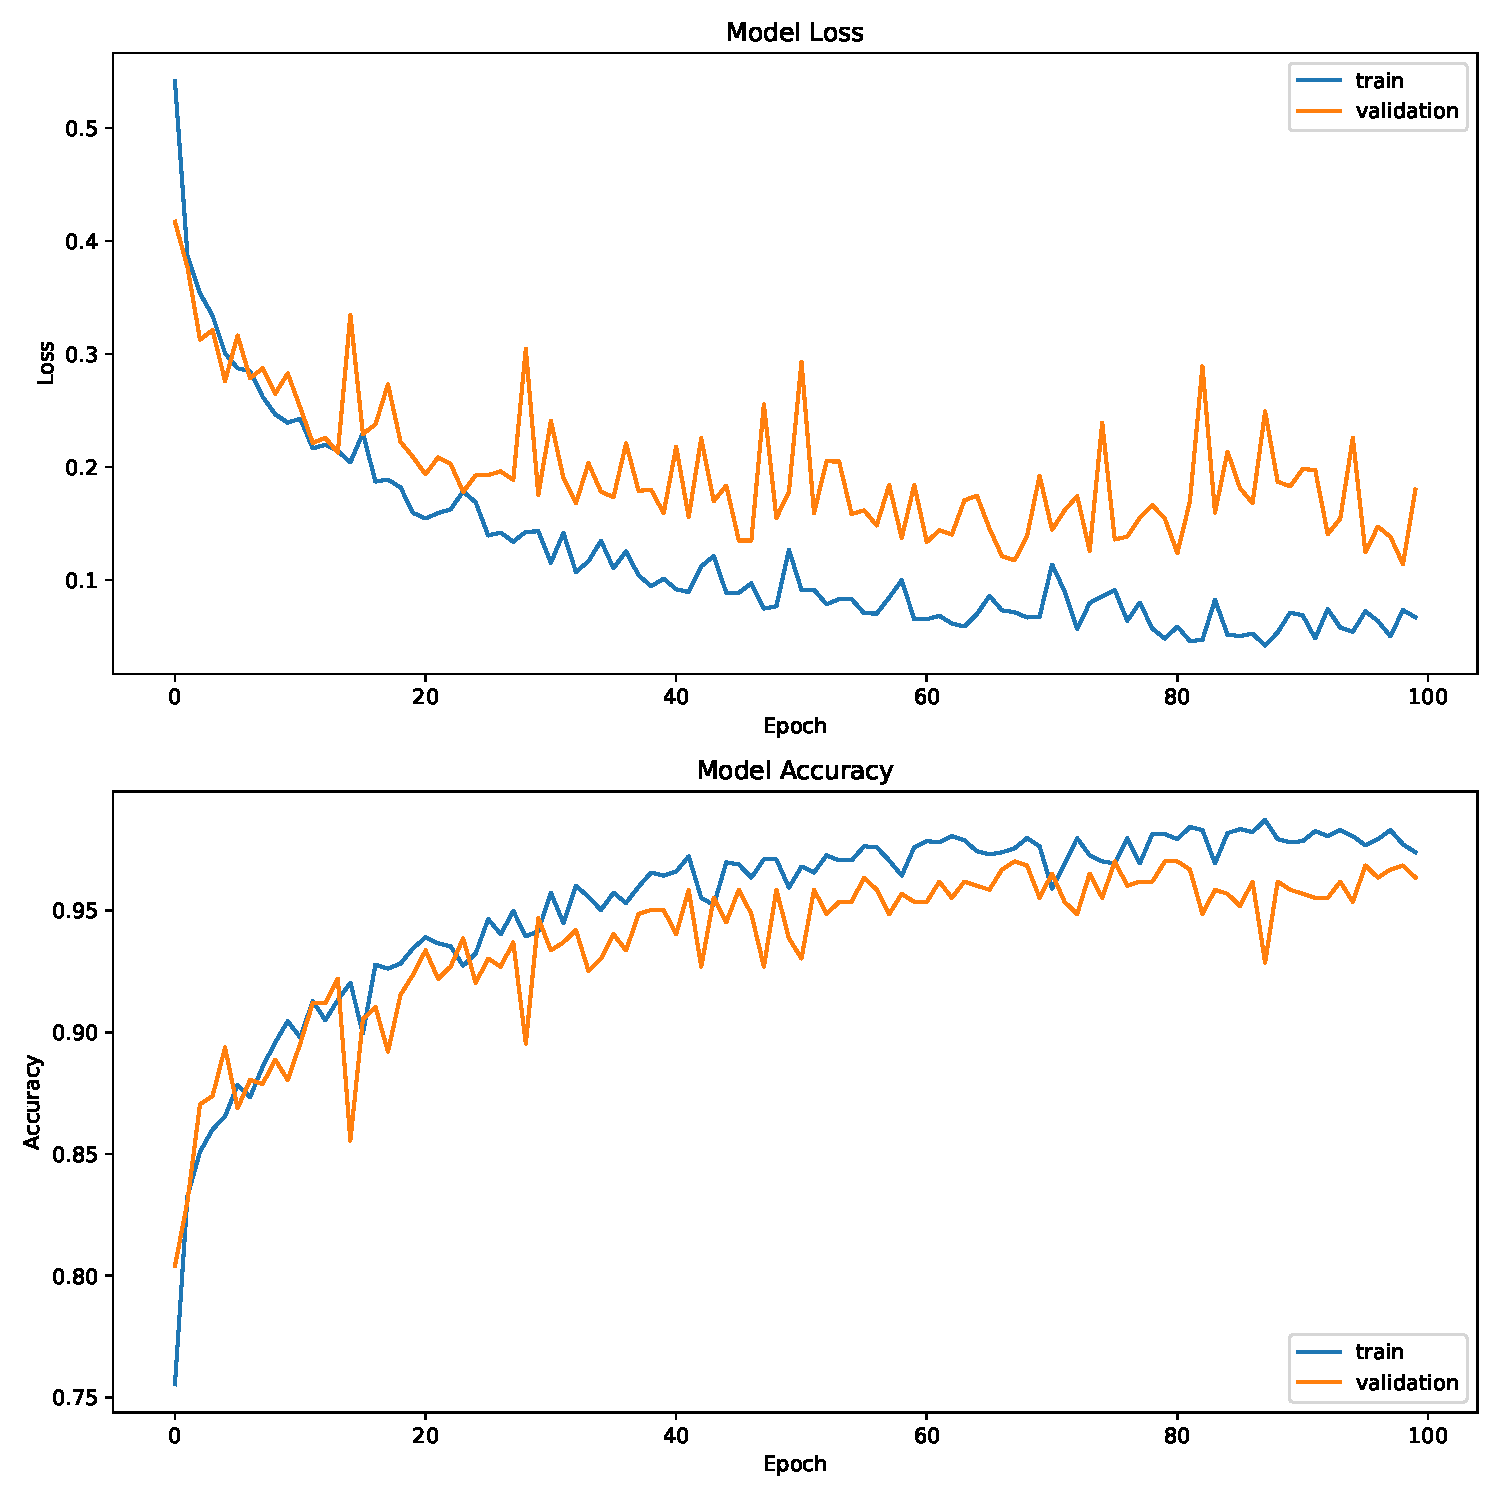
\includegraphics[width=.65\textwidth]{plots/history.pdf}
    \caption{Accuracy- and loss-curves for the final CNN after the hyperparameter optimization.}
    \label{fig:learningCurveFinal}
\end{figure}
The loss curves show that the model does not overfit as much as the initial model, even after 100 epochs, but it also shows that there is still a difference between the training and the validation loss.
As it stays constant, the model is not overfitting more with more epochs. 
This difference, however, is lower than in the initial model, indicating that the hyperparameter optimization was successful.
It can also be seen that the validation loss curve has some peaks, which can be explained by the low amount of data available, as the validation loss is calculated on a smaller dataset of 602 samples.
Similar behaviour can be seen in the accuracy curves, with the validation accuracy being lower than the training accuracy.
The difference between the training and the validation accuracy is also smaller than in the initial model.
The overall accuracy of the model is higher than in the initial model, showing that the hyperparameter optimization was successful.

The confusion matrix for the final model is shown in figure \ref{fig:confusionMatrixFinal}.
It shows similar behaviour as in the final model, with the model classifying more benign tumours as malignant than the other way around.
The amount of tumours that are misclassified, however, is lower than in the initial model.
The metrics for the final model are shown in the summary below (\ref{eq:metricsFinalCNN}). \newline
\begin{wrapfigure}{r}{5cm}
    \centering
    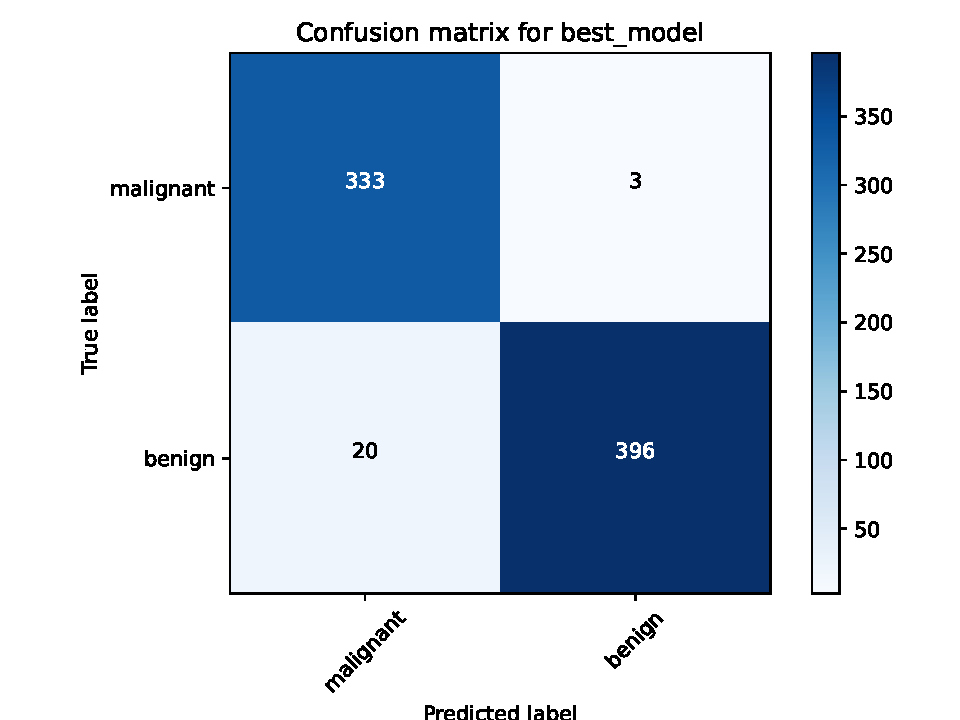
\includegraphics[width=.48\textwidth]{plots/confusion_matrix_best_model.pdf}
    \caption{Confusion matrix for the final CNN after the hyperparameter optimization.}
    \label{fig:confusionMatrixFinal}
\end{wrapfigure}
\noindent
It can be seen that all of the metrics have improved compared to the initial model.
The biggest reason for this improvement is the increase in runtime from 30 to 100 epochs.
But as the initial model was already overfitting at 30 epochs, it made sense to first optimize the hyperparameters as the initial model could just adjust the weights to the training data therefore remembering it.
As the final model has shown a significant improvement in the overfitting, the results are more reliable than in the initial model. \newline
\begin{align}
    \label{eq:metricsFinalCNN}
    \begin{split}
        \text{recall} &= 0.9519, \\
        \text{accuracy} &= 0.9694, \\
        \text{precision} &= 0.9925, \\
        \text{f1-score} &= 0.9718, \\
        R^2\text{-score} &= 0.8763, \\
        \text{Mean Squared Error} &= 0.0306.
    \end{split}
\end{align}
% The recall value of 95.19\% is much better than in the initial model. 
% The improvement in the recall value is the most important as it is the metric that is most important for a medical application.
% The accuracy has improved to 96.94\%.
% As said before, the recall value is the most important metric for a medical application.
The recall value of 95.19\% is much better than in the initial model.
% The accuracy has improved to 96.94\%. 
% The precision value of 99.25\% is very high and the F1-score of 97.18\% is also very good.
% The $R^2$-score of 87.63\% is also a good value, as it means that the model is off by 12.37\%. \newline
It can be seen that all of the metrics have improved compared to the initial model.
Most importantly, the recall value is much better than in the initial model and the mean squared error is lower.
The $R^2$-score of 87.63\% is also a good value, as the model regresses better to the actual values.
% As all of the metrics have improved while the model is not overfitting as much as in the initial model, the final model is a significant improvement over the initial model.
The final model is a significant improvement over the initial model as all of the metrics have improved while the model is not overfitting as much as in the initial model.
